\section{The case of small and medium dimension}\label{h1-sec}

In this section we establish lower bounds for $M_k$ (and related quantities, such as $M_{k,\eps}$) both for small values of $k$ (in particular, $k=3$ and $k=4$) and medium values of $k$ (in particular, $k=50$ and $k=54$).  Specifically, we will establish Theorem \ref{mlower}(vii), Theorem \ref{mke-lower}, and Theorem \ref{piece}.

\subsection{Bounding \texorpdfstring{$M_k$}{Mk} for medium \texorpdfstring{$k$}{k}}

We begin with the problem of lower bounding $M_k$.  We first formalize an observation\footnote{The arguments in \cite{maynard-new} are rigorous under the assumption of a positive eigenfunction as in Corollary \ref{ef}, but the existence of such an eigenfunction remains open for $k \geq 3$.} of Maynard \cite{maynard-new} that one may restrict without loss of generality to symmetric functions:

\begin{lemma}  For any $k \geq 2$, one has
$$ M_k \coloneqq \sup \frac{k J_1(F)}{I(F)}$$
where $F$ ranges over \emph{symmetric} square-integrable functions on ${\mathcal R}_k$ that are not identically zero.
\end{lemma}

\begin{proof}  Firstly, observe that if one replaces a square-integrable function $F: [0,+\infty)^k \to \R$ with its absolute value $|F|$, then $I(|F|) = I(F)$ and $J_i(|F|) \geq J_i(F)$.  Thus one may restrict the supremum in \eqref{mk4} to non-negative functions without loss of generality.  We may thus find a sequence $F_n$ of square-integrable non-negative functions on ${\mathcal R}_k$, normalized so that $I(F_n)=1$, and such that $\sum_{i=1}^k J_i(F_n) \to M_k$ as $n \to \infty$.

Now let
$$\overline{F_n}(t_1,\dots,t_k) \coloneqq \frac{1}{k!} \sum_{\sigma \in S_k} F_n( t_{\sigma(1)},\dots,t_{\sigma(k)} )$$
be the symmetrization of $F_n$.  Since the $F_n$ are non-negative with $I(F_n)=1$, we see that
$$ I( \overline{F_n} ) \geq I( \frac{1}{k!} F_n ) = \frac{1}{(k!)^2}$$
and so $I(\overline{F_n})$ is bounded away from zero.  Also, from \eqref{mk4}, we know that the quadratic form
$$ Q(F) \coloneqq M_k I(F) - \sum_{i=1}^k J_i(F)$$
is positive semi-definite and is also invariant with respect to symmetries, and so from the triangle inequality for inner product spaces we conclude that
$$ Q( \overline{F_n} ) \leq Q( F_n ).$$
By construction, $Q(F_n)$ goes to zero as $n \to \infty$, and thus $Q(\overline{F_n})$ also goes to zero.  We conclude that
$$ \frac{k J_1(\overline{F_n})}{I(\overline{F_n})} = \frac{\sum_{i=1}^k J_i(\overline{F_n})}{I(\overline{F_n})} \to M_k$$
as $n \to \infty$, and so
$$ M_k \geq \sup \frac{k J_1(F)}{I(F)}.$$
The reverse inequality is immediate from \eqref{mk4}, and the claim follows.
\end{proof}

To establish a lower bound of the form $M_k > C$ for some $C > 0$, one thus seeks to locate a symmetric function $F: [0,+\infty)^k \to \R$ supported on ${\mathcal R}_k$ such that
\begin{equation}\label{kjaf}
 k J_1(F) > C I(F).
\end{equation}
To do this numerically, we follow \cite{maynard-new} (see also \cite{gpy} for some related ideas) and can restrict attention to functions $F$ that are linear combinations
$$ F = \sum_{i=1}^n a_i b_i$$
of some explicit finite set $b_1,\dots,b_n: [0,+\infty)^k \to \R$ supported on ${\mathcal R}_k$, and some real scalars $a_1,\dots,a_n$ that we may optimize in.  The condition \eqref{kjaf} then may be rewritten as
\begin{equation}\label{ama}
 \mathbf{a}^T \mathbf{M}_2 \mathbf{a} - C \mathbf{a}^T \mathbf{M}_1 \mathbf{a} > 0
\end{equation}
where $\mathbf{a}$ is the vector
$$ \mathbf{a} \coloneqq \begin{pmatrix} a_1 \\ \vdots \\ a_n \end{pmatrix}
$$
and $\mathbf{M}_1,\mathbf{M}_2$ are the real symmetric and positive semi-definite $n \times n$ matrices
\begin{align}\label{Eq:M1}
\mathbf{M}_1 &= \left( \int_{\R^k} b_i(t_1,\dots,t_k) b_j(t_1,\dots,t_k)\ dt_1 \dots dt_k \right)_{1 \leq i,j \leq n} \\\label{Eq:M2}
\mathbf{M}_2 &= \left( k \int_{\R^{k+1}} b_i(t_1,\dots,t_k) b_j(t_1,\dots,t_{k-1},t'_k)\ dt_1 \dots dt_k dt'_k\right)_{1 \leq i,j \leq n}.
\end{align}
If the $b_1,\dots,b_n$ are linearly independent in $L^2({\mathcal R}_k)$, then $\mathbf{M}_1$ is strictly positive definite, and (as observed in \cite[Lemma 8.3]{maynard-new}), one can find $\mathbf{a}$ obeying \eqref{ama} if and only if the largest eigenvalue of $\mathbf{M}_2 \mathbf{M}_1^{-1}$ exceeds $C$.  This is a criterion that can be numerically verified for medium-sized values of $n$, if the $b_1,\dots,b_n$ are chosen so that the matrix coefficients of $\mathbf{M}_1,\mathbf{M}_2$ are explicitly computable.

In order to facilitate computations, it is natural to work with bases $b_1,\dots,b_n$ of symmetric polynomials.  We have the following basic integration identity:

\begin{lemma}[Beta function identity]\label{bfi}  For any non-negative $a,a_1,\dots,a_k$, we have
$$ \int_{{\mathcal R}_k} (1-t_1-\dots-t_k)^a t_1^{a_1} \dots t_k^{a_k}\ dt_1 \dots dt_k = \frac{\Gamma(a+1) \Gamma(a_1+1) \dots \Gamma(a_k+1)}{\Gamma(a_1+\dots+a_k+k+a+1)}$$
where $\Gamma(s) := \int_0^\infty t^{s-1} e^{-t}\ dt$ is the Gamma function.  In particular, if $a_1,\dots,a_k$ are natural numbers, then
$$ \int_{{\mathcal R}_k} (1-t_1-\dots-t_k)^a t_1^{a_1} \dots t_k^{a_k}\ dt_1 \dots dt_k = \frac{a! a_1! \dots a_k!}{(a_1+\dots+a_k+k+a)!}.$$
\end{lemma}

\begin{proof}
Since
$$ \int_{{\mathcal R}_k} (1-t_1-\dots-t_k)^a t_1^{a_1} \dots t_k^{a_k}\ dt_1 \dots dt_k = a \int_{{\mathcal R}_{k+1}} t_1^{a_1} \dots t_k^{a_k} t_{k+1}^{a-1}\ dt_1 \dots dt_{k+1}$$
we see that to establish the lemma it suffices to do so in the case $a=0$.

If we write
$$ X := \int_{t_1+\dots+t_k=1} t_1^{a_1} \dots t_k^{a_k}\ dt_1 \dots dt_{k-1}$$
then by homogeneity we have
$$ r^{a_1+\dots+a_k+k-1} X = \int_{t_1+\dots+t_k=r} t_1^{a_1} \dots t_k^{a_k}\ dt_1 \dots dt_{k-1}$$
for any $r > 0$, and hence on integrating $r$ from $0$ to $1$ we conclude that
$$ \frac{X}{a_1+\dots+a_k+k} = \int_{{\mathcal R}_k} t_1^{a_1} \dots t_k^{a_k}\ dt_1 \dots dt_k.$$
On the other hand, if we multiply by $e^{-r}$ and integrate $r$ from $0$ to $\infty$, we obtain instead
$$ \int_0^\infty r^{a_1+\dots+a_k+k-1} X e^{-r}\ dr = \int_{[0,+\infty)^k} t_1^{a_1} \dots t_k^{a_k} e^{-t_1-\dots-t_k}\ dt_1 \dots dt_k.$$
Using the definition of the Gamma function, this becomes
$$ \Gamma(a_1+\dots+a_k+k) X = \Gamma(a_1+1) \dots \Gamma(a_k+1)$$
and the claim follows.
\end{proof}

Define a \emph{signature} to be a non-increasing sequence $\alpha = (\alpha_1,\alpha_2,\dots,\alpha_k)$ of natural numbers; for brevity we omit zeroes, thus for instance if $k=6$, then $(2,2,1,1,0,0)$ will be abbreviated as $(2,2,1,1)$.  The number of non-zero elements of $\alpha$ will be called the \emph{length} of the signature $\alpha$, and as usual the \emph{degree} of $\alpha$ with be $\alpha_1+\dots+\alpha_k$.  For each signature $\alpha$, we then define the symmetric polynomials $P_\alpha = P^{(k)}_\alpha$ by the formula
$$
P_\alpha(t_1,\dots,t_k) = \sum_{a: s(a)=\alpha} t_1^{a_1} \dots t_k^{a_k}$$
where the summation is over all tuples $a = (a_1,\dots,a_k)$ whose non-increasing rearrangement $s(a)$ is equal to $\alpha$.  Thus for instance
\begin{align*}
P_{(1)}(t_1,\dots,t_k) &= t_1 + \dots + t_k \\
P_{(2)}(t_1,\dots,t_k) &= t_1^2 + \dots + t_k^2 \\
P_{(1,1)}(t_1,\dots,t_k) &= \sum_{1 \leq i < j \leq k} t_i t_j \\
P_{(2,1)}(t_1,\dots,t_k) &= \sum_{1 \leq i < j \leq k} t_i^2 t_j + t_i t_j^2
\end{align*}
and so forth.  Clearly, the $P_\alpha$ form a linear basis for the symmetric polynomials of $t_1,\dots,t_k$.  Observe that if $\alpha = (\alpha',1)$ is a signature containing $1$, then one can express $P_\alpha$ as $P_{(1)} P_{\alpha'}$ minus a linear combination of polynomials $P_\beta$ with the length of $\beta$ less than that of $\alpha$.  This implies that the functions $P_{(1)}^a P_\alpha$, with $a \geq 0$ and $\alpha$ avoiding $1$, are also a basis for the symmetric polynomials.  Equivalently, the functions $(1-P_{(1)})^a P_\alpha$ with $a \geq 0$ and $\alpha$ avoiding $1$ form a basis.

After extensive experimentation, we have discovered that a good basis $b_1,\dots,b_n$ to use for the above problem comes by setting the $b_i$ to be all the symmetric polynomials of the form $(1-P_{(1)})^a P_\alpha$, where $a \geq 0$ and $\alpha$ consists entirely of even numbers, whose total degree $a + \alpha_1+\dots +\alpha_k$ is less than or equal to some chosen threshold $d$.  For such functions, the coefficients of $\mathbf{M}_1,\mathbf{M}_2$ can be computed exactly using Lemma \ref{bfi}.

More explicitly, first we quickly compute a look-up table for the structure constants $c_{\alpha,\beta,\gamma}\in \Z$ derived from simple products of the form
\[
P_{\alpha}P_{\beta}=\sum_{\gamma}c_{\alpha,\beta,\gamma}P_{\gamma}
\]
where $\deg(\alpha)+\deg(\beta)\leq d$.  Using this look-up table we rewrite the integrands of the entries of the matrices in (\ref{Eq:M1}) and (\ref{Eq:M2}) as integer linear combinations of nearly ``pure'' monomials of the form $(1-P_{(1)})^a t_1^{a_1}\dots t_k^{a_k}$.  We then calculate the entries of $\mathbf{M}_1$ and $\mathbf{M}_2$, as exact rational numbers, using Lemma \ref{bfi}.

We next run a generalized eigenvector routine on (real approximations to) $\mathbf{M}_1$ and $\mathbf{M}_2$ to find a vector $\mathbf{a}'$ which nearly maximize the quantity$C$ in (\ref{ama}).  Taking a rational approximation $\mathbf{a}$ to $\mathbf{a}'$, we then do the quick (and exact) arithmetic to verify that (\ref{ama}) holds for some constant $C>4$.  This generalized eigenvector routine is time-intensive when the sizes of $\mathbf{M}_1$ and $\mathbf{M}_2$ are large (say, bigger than $1500\times 1500$), and in practice  is the most computationally intensive step of our calculation.  When one does not care about an exact arithmetic proof that $C>4$, instead one can run a test for positive-definiteness for the matrix $C\mathbf{M}_1-\mathbf{M}_2$, which is usually much faster and less RAM intensive.

Using this method, we were able to demonstrate $M_{54} > 4.00238$, thus establishing Theorem \ref{mlower}(vii).  We took $d=23$ and imposing the restriction on signatures $\alpha$ that they be composed only of even numbers. It is likely that $d=22$ would suffice in the absence of this restriction on signatures, but we found that the gain in $M_{54}$ from lifting this restriction is typically only in the region of $0.005$, whereas the execution time is increased by a large factor. We do not have a good understanding of why this particular restriction on signatures is so inexpensive in terms of the trade-off between the accuracy of $M$-values and computational complexity.  The total run-time for this computation was under one hour.


We now describe a second choice for the basis elements $b_1,\dots,b_n$, which uses the Krylov subspace method; it gives faster and more efficient numerical results than the previous basis, but does not seem to extend as well to more complicated variational problems such as $M_{k,\eps}$.  We introduce the linear operator ${\mathcal L}: L^2({\mathcal R}_k) \to L^2({\mathcal R}_k)$ defined by
$$ {\mathcal L} f( t_1,\dots,t_k) \coloneqq \sum_{i=1}^k \int_0^{1-t_1-\dots-t_{i-1}-t_{i+1}-\dots-t_k} f(t_1,\dots,t_{i-1},t'_i,t_{i+1},\dots,t_k)\ dt'_i.$$
This is a self-adjoint and positive semi-definite operator on $L^2({\mathcal R}_k)$.  For symmetric $b_1,\dots,b_n \in L^2({\mathcal R}_k)$, one can then write
\begin{align*}
\mathbf{M}_1 &= \left( \langle b_i, b_j \rangle \right)_{1 \leq i,j \leq n} \\
\mathbf{M}_2 &= \left( \langle {\mathcal L} b_i, b_j \rangle \right)_{1 \leq i,j \leq n}.
\end{align*}
If we then choose
$$ b_i \coloneqq {\mathcal L}^{i-1} 1$$
where $1$ is the unit constant function on ${\mathcal R}_k$, then the matrices $\mathbf{M}_1,\mathbf{M}_2$ take the Hankel form
\begin{align*}
\mathbf{M}_1 &= \left( \langle {\mathcal L}^{i+j-2} 1, 1 \rangle \right)_{1 \leq i,j \leq n} \\
\mathbf{M}_2 &= \left( \langle {\mathcal L}^{i+j-1} 1, 1 \rangle \right)_{1 \leq i,j \leq n},
\end{align*}
and so can be computed entirely in terms of the $2n$ numbers $\langle {\mathcal L}^i 1, 1 \rangle$ for $i=0,\dots,2n-1$.

The operator ${\mathcal L}$ maps symmetric polynomials to symmetric polynomials; for instance, one has
\begin{align*}
{\mathcal L} 1 &= k - (k-1) 	P_{(1)} \\
{\mathcal L} P_{(1)} &= \frac{k}{2} - \frac{k-1}{2} P_{(2)} - (k-2) P_{(1,1)}
\end{align*}
and so forth.  From this and Lemma \ref{bfi}, the quantities $\langle {\mathcal L}^i 1, 1 \rangle$ are explicitly computable rational numbers; for instance, one can calculate
\begin{align*}
\langle 1, 1 \rangle &= \frac{1}{k!} \\
\langle {\mathcal L} 1, 1\rangle &= \frac{2k}{(k+1)!} \\
\langle {\mathcal L}^2 1, 1\rangle &= \frac{k (5k+1)}{(k+2)!} \\
\langle {\mathcal L}^3 1, 1\rangle &= \frac{2k^2 (7k+5)}{(k+3)!}
\end{align*}
and so forth.

With Maple, we were able to compute $\langle {\mathcal L}^i 1, 1 \rangle$ for $i \leq 50$ and $k \leq 100$, leading to lower bounds on $M_k$ for these values of $k$, a selection of which are given in Table \ref{tab}.

\begin{table}
\centering
 \caption{Selected lower bounds on $M_k$ obtained from the Krylov subspace method, with the $\frac{k}{k-1} \log k$ upper bound displayed for comparison.}
 \label{tab}
  \begin{tabular}{lll}
	% D{.}{.}{4.0} D{.}{.}{8.0} D{.}{.}{8.0} D{.}{.}{9.0}}
   \toprule
     $k$    & Lower bound on $M_k$   & $\frac{k}{k-1} \log k$   \\
   \midrule
           2 & 1.38593            & 1.38629                \\
           3 & 1.64644            & 1.64791              \\ [0.5ex]
           4 & 1.84540  	        & 1.84839             \\
           5 & 2.00714  	        & 2.01179             \\ [0.5ex]
          10 & 2.54547            & 2.55842              \\
				  20 & 3.12756            & 3.15340              \\  [0.5ex]
          30 & 3.48313            & 3.51848              \\
          40 & 3.73919            & 3.78346            \\  [0.5ex]
          50 & 3.93586            & 3.99186              \\
          53 & 3.98621            & 4.04664            \\  [0.5ex]
          54 & 4.00223            & 4.06424            \\
          60 & 4.09101            & 4.16374            \\  [0.5ex]
				 100 & 4.46424            & 4.65168           \\
   \bottomrule
  \end{tabular}
\end{table}


\subsection{Bounding \texorpdfstring{$M_{k,\eps}$}{Mk,epsilon} for medium \texorpdfstring{$k$}{k}}\label{mkeps-sec}

When bounding $M_{k,\eps}$, we have not been able to implement the Krylov method, because the analogue of ${\mathcal L}^i 1$ in this context is piecewise polynomial instead of polynomial, and we were only able to compute it explicitly for very small values of $i$, such as $i=1,2,3$, which are insufficient for good numerics.  Thus, we rely on the previously discussed approach, in which symmetric polynomials are used for the basis functions.  Instead of computing integrals over the region ${\mathcal R}_k$ we pass to the regions $(1\pm \varepsilon)\mathcal{R}_k$.  In order to apply Lemma \ref{bfi} over these regions, this necessitates working with a slightly different basis of polynomials.  We chose to work with those polynomials of the form $(1+\varepsilon-P_{(1)})^a P_{\alpha}$, where $\alpha$ is a signature with no 1's.  Over the region $(1+\varepsilon)\mathcal{R}_k$, a single change of variables converts the needed integrals into those of the form in Lemma \ref{bfi}, and we can then compute the entries of $\mathbf{M}_1$.

On the other hand, over the region $(1-\varepsilon)\mathcal{R}_k$ we instead want to work with polynomials of the form $(1-\varepsilon-P_{(1)})^aP_{\alpha}$.  Since $(1+\varepsilon-P_{(1)})^a=(2\varepsilon +(1-\varepsilon-P_{(1)}))^a$, an expansion using the binomial theorem allows us to convert from our given basis to polynomials of the needed form.

With these modifications, and calculating as in the previous section, we find that $M_{50,1/25}>4.00124$ if $d=25$ and $M_{50,1/25}>4.0043$ if $d=27$, thus establishing Theorem \ref{mlower}(i).  As before, we found it optimal to restrict signatures to contain only even entries, which greatly reduced execution time while only reducing $M$ by a few thousandths.

One surprising additional computational difficulty introduced by allowing $\varepsilon>0$ is that the ``complexity'' of $\varepsilon$ as a rational number affects the run-time of the calculations.  We found that choosing $\varepsilon=1/m$ (where $m\in \Z$ has only small prime factors) reduces this effect.

A similar argument gives $M_{51,1/50} > 4.00156$, thus establishing Theorem \ref{mke-lower}(xiii). In this case our polynomials were of maximum degree $d= 22$.

Code and data for these calculations may be found at 

\centerline{{\tt www.dropbox.com/sh/0xb4xrsx4qmua7u/WOhuo2Gx7f/Polymath8b}.}

\subsection{Bounding \texorpdfstring{$M_{4,\eps}$}{M4,0.18}}\label{4d}

We now prove Theorem \ref{mke-lower}(xii'), which can be established by a direct numerical calculation.  We introduce the explicit function $F: [0,+\infty)^4 \to \R$ defined by
$$ F(t_1,t_2,t_3,t_4) \coloneqq (1 - \alpha (t_1+t_2+t_3+t_4)) 1_{t_1+t_2+t_3+t_4 \leq 1+\eps}$$
with $\eps \coloneqq 0.168$ and $\alpha \coloneqq 0.784$.  As $F$ is symmetric in $t_1,t_2,t_3,t_4$, we have $J_{i,1-\eps}(F) = J_{1,1-\eps}(F)$, so to show Theorem \ref{mke-lower}(xii') it will suffice to show that
\begin{equation}\label{jf}
 \frac{4 J_{1,1-\eps}(F)}{I(F)} > 2.00558.
\end{equation}
By making the change of variables $s=t_1+t_2+t_3+t_4$ we see that
\begin{align*}
I(F) &= \int_{t_1+t_2+t_3+t_4 \leq 1+\eps} (1-\alpha(t_1+t_2+t_3+t_4))^2\ dt_1 dt_2 dt_3 dt_4 \\
&= \int_0^{1+\eps} (1-\alpha s)^2 \frac{s^3}{3!}\ ds\\
&= \alpha^2 \frac{(1+\eps)^6}{36} - \alpha \frac{(1+\eps)^5}{15} + \frac{(1+\eps)^4}{24} \\
&= 0.00728001347\dots
\end{align*}
and similarly by making the change of variables $u = t_1+t_2+t_3$
\begin{align*}
J_{1,1-\eps}(F) &= \int_{t_1+t_2+t_3 \leq 1-\eps} (\int_0^{1+\eps-t_1-t_2-t_3} (1-\alpha(t_1+t_2+t_3+t_4))\ dt_4)^2 dt_1 dt_2 dt_3 \\
&= \int_0^{1-\eps} (\int_0^{1+\eps-u} (1-\alpha(u+t_4))\ dt_4)^2 \frac{u^2}{2!} du \\
&= \int_0^{1-\eps} (1+\eps-u)^2 (1-\alpha \frac{1+\eps+u}{2})^2 \frac{u^2}{2} du  \\
&= 0.003650160667\dots
\end{align*}
and so \eqref{jf} follows.

\begin{remark}  If we use the truncated function
$$ \tilde F(t_1,t_2,t_3,t_4) \coloneqq F(t_1,t_2,t_3,t_4) 1_{t_1,t_2,t_3,t_4 \leq 1}$$
in place of $F$, and sets $\eps$ to $0.18$ instead of $0.168$, one can compute that
$$ \frac{4 J_{1,1-\eps}(\tilde F)}{I(\tilde F)} > 2.00235.$$
Thus it is possible to establish Theorem \ref{mke-lower}(xii') using a cutoff function $F'$ that is also supported in the unit cube $[0,1]^4$.  This allows for a slight simplification to the proof of $\DHL[4,2]$ assuming GEH, as one can add the additional hypothesis $S(F_{i_0})+S(G_{i_0}) < 1$ to Theorem \ref{nonprime-asym}(ii) in that case.
\end{remark}

\begin{remark} By optimising in $\eps$ and taking $F$ to be a symmetric polynomial of degree higher than $1$, one can get slightly better lower bounds for $M_{4,\eps}$; for instance setting $\eps = 5/21$ and choosing $F$ to be a cubic polynomial, we were able to obtain the bound $M_{4,\eps} \geq 2.05411$.  On the other hand, the best lower bound for $M_{3,\eps}$ that we were able to obtain was $1.91726$ (taking $\eps = 56/113$ and optimizing over cubic polynomials).  Again, see {\tt www.dropbox.com/sh/0xb4xrsx4qmua7u/WOhuo2Gx7f/Polymath8b} for the relevant code and data.
\end{remark}

\subsection{Three-dimensional cutoffs}\label{3d}

In this section we establish Theorem \ref{piece}.  We relabel the variables $(t_1,t_2,t_3)$ as $(x,y,z)$, thus our task is to locate a piecewise polynomial function
$F: [0,+\infty)^3 \to \R$ supported the simplex
$$ R := \left\{ (x,y,z) \in [0,+\infty)^3: x+y+z \leq \frac{3}{2}\right\}$$
and symmetric in the $x,y,z$ variables, obeying the vanishing marginal condition
\begin{equation}\label{fmor}
\int_0^\infty F(x,y,z)\ dz = 0
\end{equation}
whenever $x,y \geq 0$ with $x+y > 1+\eps$, and such that
\begin{equation}\label{tt1}
J(F) > 2 I(F)
\end{equation}
where
\begin{equation}\label{jf-def}
J(F) := 3\int_{x+y \leq 1-\eps} \left(\int_0^\infty F(x,y,z)\ dz\right)^2\ dx dy
\end{equation}
and
\begin{equation}\label{if-def}
I(F) := \int_R  F(x,y,z)^2\ dx dy dz
\end{equation}
and
$$\eps := 1/4.$$

Our strategy will be as follows.  We will decompose the simplex $R$ (up to null sets) into a carefully selected set of disjoint open polyhedra $P_1,\dots,P_m$ (in fact $m$ will be $60$), and on each $P_i$ we will take $F(x,y,z)$ to be a low degree polynomial $F_i(x,y,z)$ (indeed, the degree will never exceed $3$).  The left and right-hand sides of \eqref{tt1} become quadratic functions in the coefficients of the $F_i$.  Meanwhile, the requirement of symmetry, as well as the marginal requirement \eqref{fmor}, imposes some linear constraints on these coefficients.  In principle, this creates a finite-dimensional quadratic program, which one can try to solve numerically.  However, to make this strategy practical, one needs to keep the number of linear constraints imposed on the coefficients to be fairly small, as compared with the total number of coefficients.  To achieve this, the following properties on the polynomials $P_i$ are desirable:

\begin{itemize}
\item (Symmetry) If $P_i$ is a polytope in the partition, then every reflection of $P_i$ formed by permuting the $x,y,z$ coordinates should also lie in the partition.
\item (Graph structure) Each polytope $P_i$ should be of the form
\begin{equation}\label{qi-form}
\{ (x,y,z): z \in Q_i; a_i(x,y) < z < b_i(x,y)\},
\end{equation}
where $a_i(x,y), b_i(x,y)$ are linear forms and $Q_i$ is a polygon.
\item (Epsilon splitting)  Each $Q_i$ is contained in one of the regions $\{ (x,y): x+y < 1-\eps\}$, $\{ (x,y): 1-\eps < x+y < 1+\eps \}$, or $\{ (x,y): 1+\eps < x+y < 3/2 \}$.
\end{itemize}

Observe that the vanishing marginal condition \eqref{fmor} now takes the form
\begin{equation}\label{vanish}
 \sum_{i: (x,y) \in Q_i} \int_{a_i(x,y)}^{b_i(x,y)} F_i(x,y,z)\ dz = 0
\end{equation}
for every $x,y > 0$ with $x+y > 1+\eps$.  If the set $\{i: (x,y) \in Q_i\}$ is fixed, then the left-hand side of \eqref{vanish} is a polynomial in $x,y$ whose coefficients depend linearly on the coefficients on the $F_i$, and thus \eqref{vanish} imposes a set of linear conditions on these coefficients for each possible set $\{ i: (x,y) \in Q_i\}$ with $x+y > 1+\eps$.

Now we describe the partition we will use.  This partition can in fact be used for all $\eps$ in the interval $[1/4,1/3]$, but the endpoint $\eps = 1/4$ has some simplifications which allowed for reasonably good numerical results.  To obtain the symmetry property, it is natural to split $R$ (modulo null sets) into six polyhedra $R_{xyz}, R_{xzy}, R_{yxz}, R_{yzx}, R_{zxy}, R_{zyx}$, where
\begin{align*}
 R_{xyz} &:= \{(x,y,z)\in R\ :\ x+y < y+z < z+x\} \\
&= \{(x,y,z): 0 < y < x < z; x+y+z \leq 3/2 \}
\end{align*}
and the other polyhedra are obtained by permuting the indices $x,y,z$, thus for instance
\begin{align*}
R_{yxz} &:= \{(x,y,z)\in R\ :\ y+x < x+z < z+y\} \\
&= \{(x,y,z): 0 < x < y < z; x+y+z \leq 3/2 \}.
\end{align*}
%The polytope $R_{xyz}$ is a tetrahedron with vertices $(0,0,0), (0,0,3/2), (3/4,0,3/4), (1/2,1/2,1/2)$, and similarly for the other five polyhedra.

To obtain the epsilon splitting property, we decompose $R_{xyz}$ (modulo null sets) into eight sub-polytopes
\begin{align*}
A_{xyz} & =\{(x,y,z)\in R\ :\ x+y< y+z< z+x< 1-\eps\},\\
B_{xyz} & =\{(x,y,z)\in R\ :\ x+y< y+z< 1-\eps< z+x< 1+\eps\},\\
C_{xyz} & =\{(x,y,z)\in R\ :\ x+y< 1-\eps < y+z < z+x< 1+\eps\},\\
D_{xyz} & =\{(x,y,z)\in R\ :\ 1-\eps < x+y<  y+z < z+x< 1+\eps\},\\
E_{xyz} & =\{(x,y,z)\in R\ :\ x+y< y+z< 1-\eps <  1+\eps < z+x\},\\
F_{xyz} & =\{(x,y,z)\in R\ :\ x+y< 1-\eps < y+z <  1+\eps < z+x\},\\
G_{xyz} & =\{(x,y,z)\in R\ :\ x+y< 1-\eps  <  1+\eps < y+z < z+x\},\\
H_{xyz} & =\{(x,y,z)\in R\ :\ 1-\eps < x+y<  y+z < 1+\eps < z+x\};
\end{align*}
the other five polytopes $R_{xzy}, R_{yxz}, R_{yzx}, R_{zxy}, R_{zyx}$ are decomposed similarly, leading to a partition of $R$ into $6 \times 8 = 48$ polytopes.
This is almost the partition we will use; however there is a technical difficulty arising from the fact that some of the permutations of $F_{xyz}$ do not obey the graph structure property.  So we will split $F_{xyz}$ further, into the three pieces
\begin{align*}
S_{xyz} & = \{(x,y,z)\in F_{xyz}\ :\ z< 1/2+\eps\},\\
T_{xyz} & = \{(x,y,z)\in F_{xyz}\ :\ z> 1/2+\eps;x> 1/2-\eps \}, \\
U_{xyz} & = \{(x,y,z)\in F_{xyz}\ :\ x< 1/2-\eps \}.
\end{align*}
Thus $R_{xyz}$ is now partitioned into ten polytopes $A_{xyz},$ $B_{xyz},$ $C_{xyz},$ $D_{xyz}$, $E_{xyz}$, $S_{xyz}$, $T_{xyz}$, $U_{xyz}$, $G_{xyz}$, $H_{xyz}$, and similarly for permutations of $R_{xyz}$, leading to a decomposition of $R$ into $6 \times 10 = 60$ polytopes.

%Geometrically, $A_{xyz}$ is a tetrahedron with vertices $(0,0,0), (0,0,1-\eps), (1/2-\eps/2,0,1/2-\eps/2), (1/2-\eps/2,1/2-\eps/2,1/2-\eps/2)$; $B_{xyz}$ is a polytope with vertices $(1/2-\eps/2,0,1/2-\eps/2)$, $(1/2-\eps/2,1/2-\eps/2,1/2-\eps/2)$, $(1/2+\eps/2,0,1/2+\eps/2)$, $(1/2+\eps/2,1/2-3\eps/2,1/2+\eps/2)$, $(0,0,1-\eps)$, $(2\eps,0,1-\eps)$; ...

A symmetric piecewise polynomial function $F$ supported on $R$ can now be described (almost everywhere) by specifying a polynomial function $F\downharpoonright_{P}: P \to \R$ for the ten polytopes $P = A_{xyz}, B_{xyz}, C_{xyz}, D_{xyz}, E_{xyz},  S_{xyz}, T_{xyz}, U_{xyz}, G_{xyz}, H_{xyz}$, and then extending by symmetry, thus for instance
$$ F\downharpoonright_{A_{yzx}}(x,y,z) = F\downharpoonright_{A_{xyz}}(z,x,y).$$

As discussed earlier, the expressions $I(F), J(F)$ can now be written as quadratic forms in the coefficients of the $F\downharpoonright_P$, and the vanishing marginal condition \eqref{fmor} imposes some linear constraints on these coefficients.

Observe that the polytope $D_{xyz}$ and all of its permutations make no contribution to either the functional $J(F)$ or to the marginal condition \eqref{fmor}, and give a non-negative contribution to $I(F)$.  Thus without loss of generality we may assume that
$$ F\downharpoonright_{D_{xyz}} = 0.$$
However, the other nine polytopes $A_{xyz}, B_{xyz}, C_{xyz}, E_{xyz}, S_{xyz}, T_{xyz}, U_{xyz}, G_{xyz}, H_{xyz}$ have at least one permutation which gives a non-trivial contribution to either $J(F)$ or to \eqref{fmor}, and cannot be easily eliminated.

Now we compute $I(F)$.  By symmetry we have
$$ I(F) = 3! I(F \downharpoonright_{R_{xyz}} ) = 6 \sum_P I( F \downharpoonright_P ) $$
where $P$ ranges over the nine polytopes $A_{xyz}, B_{xyz}, C_{xyz}, E_{xyz}, S_{xyz}, T_{xyz}, U_{xyz}, G_{xyz}, H_{xyz}$.  A tedious but straightforward computation shows that
\begin{align*}
I(F\downharpoonright_{A_{xyz}}) & =\int_{x=0}^{1/2-\eps/2}\int_{y=0}^{x}\int_{z=x}^{1-\eps-x}F\downharpoonright_{A_{xyz}}^2\ dz\ dy\ dx \\
I(F\downharpoonright_{B_{xyz}}) &= \left(\int_{z=1/2-\eps/2}^{1/2+\eps/2}\int_{x=1-\eps-z}^{z} +\int_{z=1/2+\eps/2}^{1-\eps}\int_{x=1-\eps-z}^{1+\eps-z}\right) \int_{y=0}^{1-\eps-z}F\downharpoonright_{B_{xyz}}^2\ dy\ dx\ dz \\
I(F\downharpoonright_{C_{xyz}}) & = \left(\int_{y=0}^{1/2-3\eps/2} \int_{x=y}^{y+2\eps} + \int_{y=1/2-3\eps/2}^{1/2-\eps}\int_{x=y}^{1-\eps-y} \right) \int_{z=1-\eps-y}^{1+\eps-x} \\
&\quad + \int_{y=1/2-\eps}^{1/2-\eps/2}\int_{x=y}^{1-\eps-y}\int_{z=1-\eps-y}^{3/2-x-y} F\downharpoonright_{C_{xyz}}^2\ dz\ dx\ dy \\
I(F\downharpoonright_{E_{xyz}}) & = \int_{z=1/2+\eps/2}^{1-\eps}\int_{x=1+\eps-z}^{z}\int_{y=0}^{1-\eps-z} F\downharpoonright_{E_{xyz}}^2\ dy\ dx\ dz \\
I(F\downharpoonright_{S_{xyz}}) & =  \left(\int_{y=0}^{1/2-3\eps/2}\int_{z=1-\eps-y}^{1/2+\eps} +\int_{y=1/2-3\eps/2}^{1/2-\eps}\int_{z=y+2\eps}^{1/2+\eps} \right)\int_{x=1+\eps-z}^{1-\eps-y} F\downharpoonright_{S_{xyz}}\ dx\ dz\ dy \\
I(F\downharpoonright_{T_{xyz}}) &  = \left(\int_{z=1/2+\eps}^{1/2+2\eps}\int_{x=1+\eps-z}^{3/2-z} + \int_{z=1/2+2\eps}^{1+\eps}\int_{x=1/2-\eps}^{3/2-z}\right)\int_{y=0}^{3/2-x-z} F\downharpoonright_{T_{xyz}}^2\ dy\ dz\ dx \\
I(F\downharpoonright_{U_{xyz}}) & = \int_{x=0}^{1/2-\eps}\int_{y=0}^{x}\int_{z=1+\eps-x}^{1+\eps-y} F\downharpoonright_{U_{xyz}}\ dz\ dy\ dx\\
I(F\downharpoonright_{G_{xyz}}) & = \int_{x=0}^{1/2-\eps}\int_{y=0}^{x}\int_{z=1+\eps-y}^{3/2-x-y} F\downharpoonright_{G_{xyz}}^2\ dx\ dz\ dy
\end{align*}
and
\begin{align*}
I(F\downharpoonright_{H_{xyz}}) & =\left(\int_{x=1/2+\eps/2}^{1-\eps}\int_{y=1-\eps-x}^{3/2-2x} +\int_{x=1-\eps}^{3/4}\int_{y=0}^{3/2-2x} \right) \int_{z=x}^{3/2-x-y}\\
&\quad + \int_{x=1/2}^{1/2+\eps/2}\int_{y=1-\eps-x}^{1/2-\eps}\int_{z=1+\eps-x}^{3/2-x-y} F\downharpoonright_{H_{xyz}}^2\ dz\ dy\ dx.
\end{align*}

Now we consider the quantity $J(F)$.  Here we only have the symmetry of swapping $x$ and $y$, so that
$$ J(F) = 6 \int_{0 < y < x; x+y < 1-\eps} \left(\int_0^{3/2-x-y} F(x,y,z)\ dz\right)^2 dx dy.$$
The region of integration meets the polytopes $A_{xyz}$, $A_{yzx}$, $A_{zyx}$, $B_{xyz}$, $B_{zyx}$, $C_{xyz}$, $E_{xyz}$, $E_{zyx}$, $S_{xyz}$, $T_{xyz}$, $U_{xyz}$, and $G_{xyz}$.

Projecting these regions to the $(x,y)$-plane, we have the diagram:
\begin{center}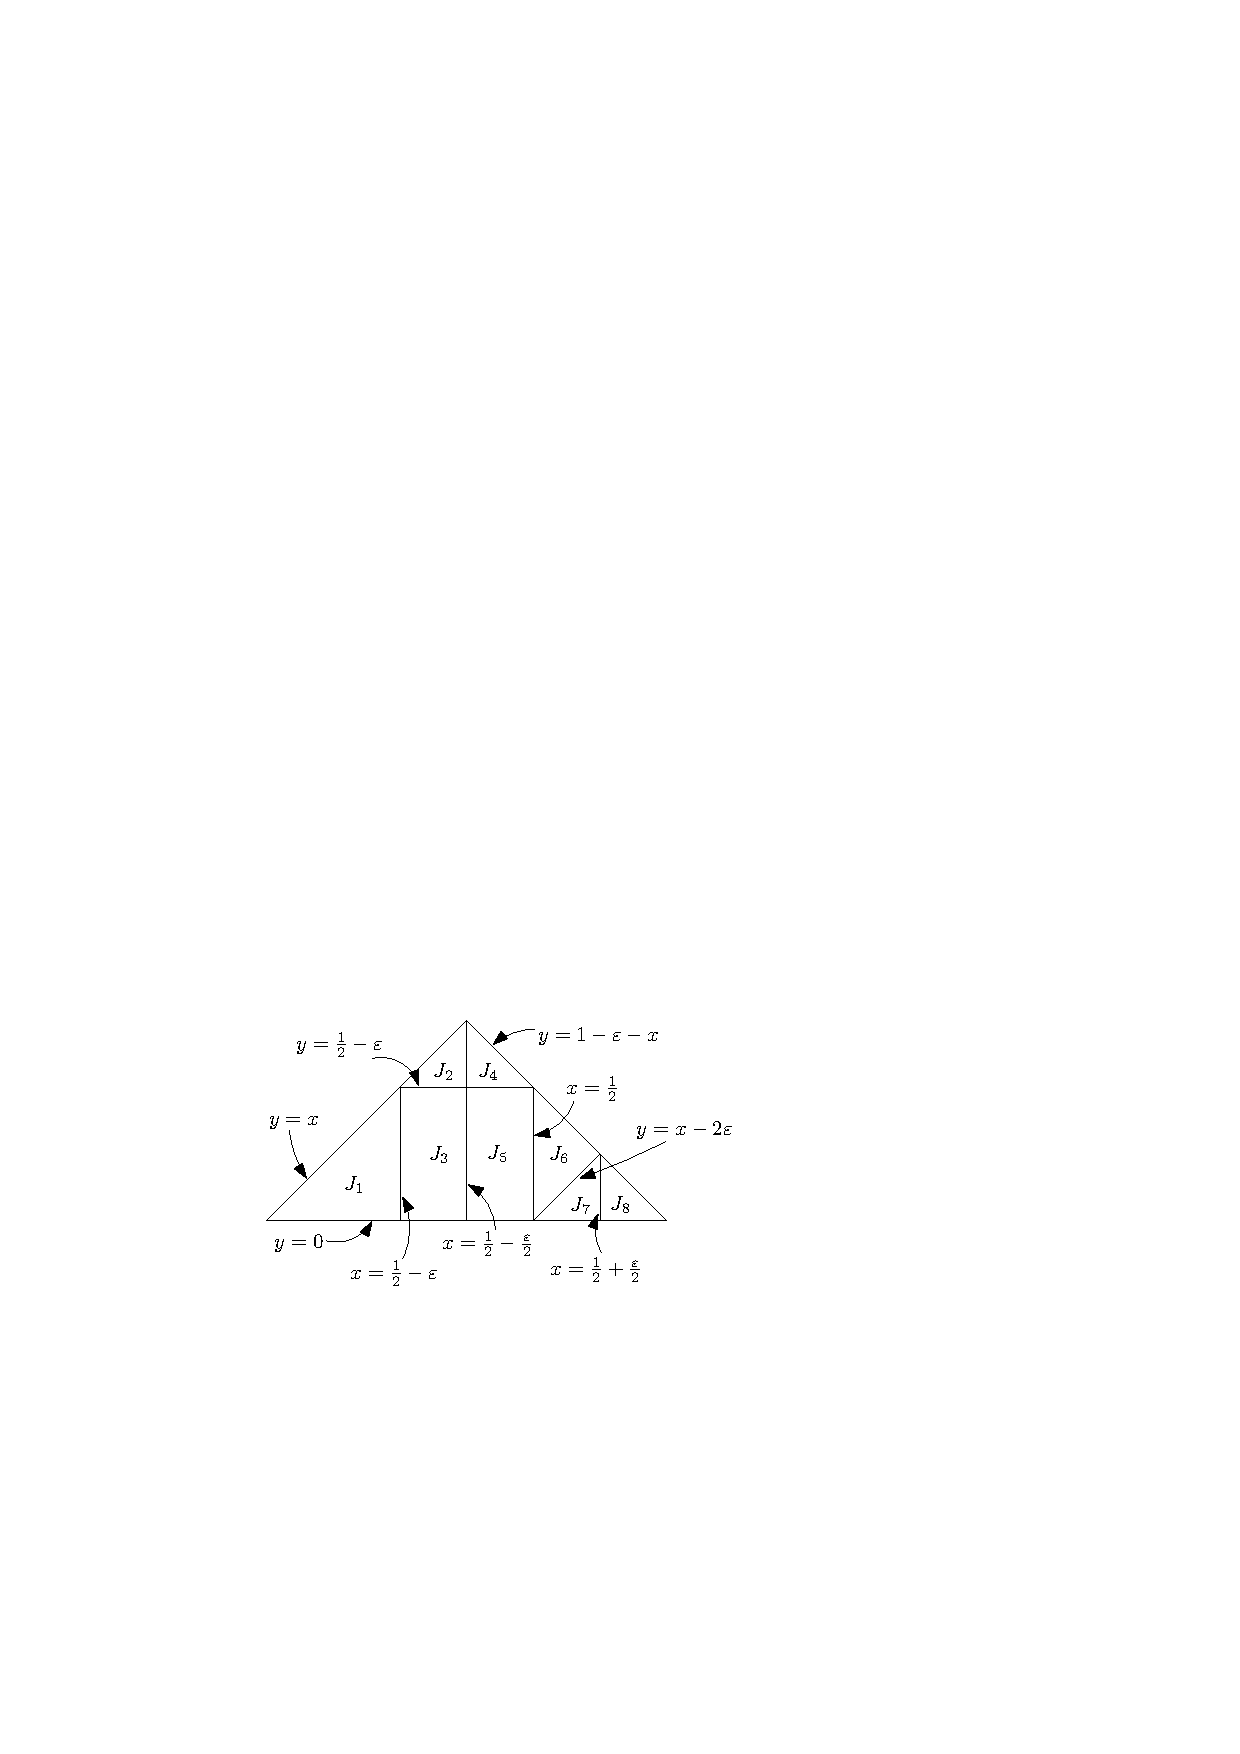
\includegraphics[scale=1.5]{xyplot.pdf}\end{center}
This diagram is drawn to scale in the case when $\varepsilon=1/4$, otherwise there is a separation between the $J_5$ and $J_7$ regions.  For each of these eight regions there are eight corresponding integrals $J_1,J_2,\ldots, J_8$, thus
$$ J = 2( J_1 + \dots + J_8).$$

We have
\begin{align*}
J_1 & =\int_{x=0}^{1/2-\eps}\int_{y=0}^{x} \left(\int_{z=0}^{y}F\downharpoonright_{A_{yzx}}+\int_{z=y}^{x}F\downharpoonright_{A_{zyx}} +\int_{z=x}^{1-\eps-x}F\downharpoonright_{A_{xyz}} +\int_{z=1-\eps-x}^{1-\eps-y}F\downharpoonright_{B_{xyz}}  \right. \\
&\quad \left. +\int_{z=1-\eps-y}^{1+\eps-x}F\downharpoonright_{C_{xyz}} + \int_{z=1+\eps-x}^{1+\eps-y}F\downharpoonright_{U_{xyz}} + \int_{z=1+\eps-y}^{3/2-x-y}F\downharpoonright_{G_{xyz}}\ dz \right)^{2}\ dy\ dx.
\end{align*}
Next comes
\begin{align*}
J_2 & =\int_{x=1/2-\eps}^{1/2-\eps/2}\int_{y=1/2-\eps}^{x} \left(\int_{z=0}^{y}F\downharpoonright_{A_{yzx}}+\int_{z=y}^{x}F\downharpoonright_{A_{zyx}}+\int_{z=x}^{1-\eps-x}F\downharpoonright_{A_{xyz}} +\int_{z=1-\eps-x}^{1-\eps-y}F\downharpoonright_{B_{xyz}}\right. \\
&\quad \left. +\int_{z=1-\eps-y}^{3/2-x-y}F\downharpoonright_{C_{xyz}}\ dz \right)^{2}\ dy\ dx.
\end{align*}
Third is the piece
\begin{align*}
J_3 & =\int_{x=1/2-\eps}^{1/2-\eps/2}\int_{y=0}^{1/2-\eps} \left(\int_{z=0}^{y}F\downharpoonright_{A_{yzx}}+\int_{z=y}^{x}F\downharpoonright_{A_{zyx}} +\int_{z=x}^{1-\eps-x}F\downharpoonright_{A_{xyz}} +\int_{z=1-\eps-x}^{1-\eps-y}F\downharpoonright_{B_{xyz}} \right. \\
&\quad \left. + \int_{z=1-\eps-y}^{1+\eps-x}F\downharpoonright_{C_{xyz}} + \int_{z=1+\eps-x}^{3/2-x-y}F\downharpoonright_{T_{xyz}}\ dz \right)^{2}\ dy\ dx.
\end{align*}

We now have dealt with all integrals involving $A_{xyz}$, and all remaining integrals pass through $B_{zyx}$.  Continuing, we have
\begin{align*}
J_4 & =\int_{x=1/2-\eps/2}^{1/2}\int_{y=1/2-\eps}^{1-\eps-x} \left(\int_{z=0}^{y}F\downharpoonright_{A_{yzx}}+\int_{z=y}^{1-\eps-x}F\downharpoonright_{A_{zyx}} +\int_{z=1-\eps-x}^{x}F\downharpoonright_{B_{zyx}} +\int_{z=x}^{1-\eps-y}F\downharpoonright_{B_{xyz}}\right. \\
&\quad \left. +\int_{z=1-\eps-y}^{3/2-x-y}F\downharpoonright_{C_{xyz}}\ dz \right)^{2}\ dy\ dx.
\end{align*}
Another component is
\begin{align*}
J_5 & = \int_{x=1/2-\eps/2}^{1/2}\int_{y=0}^{1/2-\eps} \left(\int_{z=0}^{y}F\downharpoonright_{A_{yzx}}+\int_{z=y}^{1-\eps-x}F\downharpoonright_{A_{zyx}} \right. \\
&\quad \left. +\int_{z=1-\eps-x}^{x}F\downharpoonright_{B_{zyx}} +\int_{z=x}^{1-\eps-y}F\downharpoonright_{B_{xyz}} +\int_{z=1-\eps-y}^{1+\eps-x}F\downharpoonright_{C_{xyz}} + \int_{z=1+\eps-x}^{3/2-x-y}F\downharpoonright_{T_{xyz}}\ dz \right)^{2}\ dy\ dx.
\end{align*}

The most complicated piece is
\begin{align*}
J_6 & =\left(\int_{x=1/2}^{2\eps} \int_{y=0}^{1-\eps-x} + \int_{x=2\eps}^{1/2+\eps/2}\int_{y=x-2\eps}^{1-\eps-x} \right) \left(\int_{z=0}^{y}F\downharpoonright_{A_{yzx}}+\int_{z=y}^{1-\eps-x}F\downharpoonright_{A_{zyx}} +\int_{z=1-\eps-x}^{x}F\downharpoonright_{B_{zyx}}  \right. \\
&\quad \left. +\int_{z=x}^{1-\eps-y}F\downharpoonright_{B_{xyz}} +\int_{z=1-\eps-y}^{1+\eps-x}F\downharpoonright_{C_{xyz}} + \int_{z=1+\eps-x}^{1/2+\eps}F\downharpoonright_{S_{xyz}}+ \int_{z=1/2+\eps}^{3/2-x-y}F\downharpoonright_{T_{xyz}}\ dz \right)^{2}\ dy\ dx.
\end{align*}
Here we use $\left(\int_{x=1/2}^{2\eps} \int_{y=0}^{1-\eps-x} + \int_{x=2\eps}^{1/2+\eps/2}\int_{y=x-2\eps}^{1-\eps-x} \right) f(x,y)\ dy dx$ as an abbreviation for
$$ \int_{x=1/2}^{2\eps} \int_{y=0}^{1-\eps-x} f(x,y)\ dy dx + \int_{x=2\eps}^{1/2+\eps/2}\int_{y=x-2\eps}^{1-\eps-x} f(x,y)\ dy dx.$$

We have now exhausted $C_{xyz}$.  The seventh piece is
\begin{align*}
J_7 & = \int_{x=2\eps}^{1/2+\eps/2}\int_{y=0}^{x-2\eps} \left(\int_{z=0}^{y}F\downharpoonright_{A_{yzx}}+\int_{z=y}^{1-\eps-x}F\downharpoonright_{A_{zyx}} +\int_{z=1-\eps-x}^{x}F\downharpoonright_{B_{zyx}} \right. \\
&\quad \left. +\int_{z=x}^{1+\eps-x}F\downharpoonright_{B_{xyz}} + \int_{z=1+\eps-x}^{1-\eps-y}F\downharpoonright_{E_{xyz}} + \int_{1-\eps-y}^{1/2+\eps}F\downharpoonright_{S_{xyz}}+ \int_{1/2+\eps}^{3/2-x-y}F\downharpoonright_{T_{xyz}} \ dz \right)^{2}\ dy\ dx.
\end{align*}
Finally, we have
\begin{align*}
J_8 & = \int_{x=1/2+\eps/2}^{1-\eps}\int_{y=0}^{1-\eps-x} \left(\int_{z=0}^{y}F\downharpoonright_{A_{yzx}}+\int_{z=y}^{1-\eps-x}F\downharpoonright_{A_{zyx}} +\int_{z=1-\eps-x}^{1+\eps-x}F\downharpoonright_{B_{zyx}} \right. \\
&\quad \left. + \int_{z=1+\eps-x}^{x}F\downharpoonright_{E_{zyx}} + \int_{z=x}^{1-\eps-y}F\downharpoonright_{E_{xyz}} + \int_{1-\eps-y}^{1/2+\eps}F\downharpoonright_{S_{xyz}}+ \int_{1/2+\eps}^{3/2-x-y}F\downharpoonright_{T_{xyz}}\ dz \right)^{2}\ dy\ dx.
\end{align*}

In the case $\eps=1/4$, the marginal conditions \eqref{fmor} reduce to requiring
\begin{align}
\int_{z=0}^{3/2-x-y}F\downharpoonright_{G_{yzx}}\ dz &= 0\label{m1}\\
\int_{z=0}^{y}F\downharpoonright_{G_{yzx}} +\int_{z=y}^{3/2-x-y}F\downharpoonright_{G_{zyx}}\ dz &= 0\label{m2}\\
\int_{z=0}^{1+\varepsilon-x}F\downharpoonright_{U_{yzx}} + \int_{z=1+\varepsilon-x}^{y}F\downharpoonright_{G_{yzx}} +\int_{z=y}^{3/2-x-y}F\downharpoonright_{G_{zyx}}\ dz &= 0\label{m3}\\
\int_{z=0}^{1+\varepsilon-x}F\downharpoonright_{U_{yzx}} + \int_{z=1+\varepsilon-x}^{3/2-x-y}F\downharpoonright_{G_{yzx}}\ dz &= 0\label{m4}\\
\int_{z=0}^{3/2-x-y}F\downharpoonright_{T_{yzx}}\ dz &= 0\label{m5}\\
\int_{z=0}^{1-\varepsilon-x}F\downharpoonright_{E_{yzx}} + \int_{z=1-\varepsilon-x}^{1-\varepsilon-y}F\downharpoonright_{S_{yzx}} + \int_{z=1-\varepsilon-y}^{3/2-x-y}F\downharpoonright_{H_{yzx}}\ dz &= 0.\label{m7}
\end{align}
Each of these constraints is only required to hold for some portion of the parameter space $\{ (x,y): 1+\eps \leq x+y \leq 3/2 \}$, but as the left-hand sides are all polynomial functions in $x,y$ (using the signed definite integral $\int_b^a = -\int_a^b$), it is equivalent to require that all coefficients of these polynomial functions vanish.

Now we specify $F$.  After some numerical experimentation, we have found the simplest choice of $F$ that still achieves the desired goal comes by taking $F(x,y,z)$ to be a polynomial of degree $1$ on each of $E_{xyz}$, $S_{xyz}$, $H_{xyz}$, degree $2$ on $T_{xyz}$, vanishing on $D_{xyz}$, and degree $3$ on the remaining five relevant components of $R_{xyz}$.  After solving the quadratic program, rounding, and clearing denominators, we arrive at the choice
\begin{align*}
F\downharpoonright_{A_{xyz}} &:= -66+96 x-147 x^2+125 x^3+128 y-122 x y+104 x^2 y-275 y^2+394 y^3+99 z\\
&\quad -58 x z+63 x^2 z-98 y z+51 x y z+41 y^2 z-112 z^2+24 x z^2+72 y z^2+50 z^3 \\
F\downharpoonright_{B_{xyz}} &:= -41+52 x-73 x^2+25 x^3+108 y-66 x y+71 x^2 y-294 y^2+56 x y^2+363 y^3\\
&\quad +33 z+15 x z+22 x^2 z-40 y z-42 x y z+75 y^2 z-36 z^2-24 x z^2+26 y z^2+20 z^3 \\
F\downharpoonright_{C_{xyz}} &:= -22+45 x-35 x^2+63 y-99 x y+82 x^2 y-140 y^2+54 x y^2+179 y^3 \\
F\downharpoonright_{E_{xyz}} &:= -12+8 x+32 y \\
F\downharpoonright_{S_{xyz}} &:= -6+8 x+16 y \\
F\downharpoonright_{T_{xyz}} &:= 18-30 x+12 x^2+42 y-20 x y-66 y^2-45 z+34 x z+22 z^2 \\
F\downharpoonright_{U_{xyz}} &:= 94-1823 x+5760 x^2-5128 x^3+54 y-168 x^2 y+105 y^2+1422 x z-2340 x^2 z\\
&\quad -192 y^2 z-128 z^2-268 x z^2+64 z^3 \\
F\downharpoonright_{G_{xyz}} &:= 5274-19833 x+18570 x^2-5128 x^3-18024 y+44696 x y-20664 x^2 y+16158 y^2\\
&\quad -19056 x y^2-4592 y^3-10704 z+26860 x z-12588 x^2 z+24448 y z-30352 x y z\\
&\quad -10980 y^2 z+7240 z^2-9092 x z^2-8288 y z^2-1632 z^3 \\
F\downharpoonright_{H_{xyz}} &:= 8 z.
\end{align*}
One may compute that
$$ I(F) = \frac{62082439864241}{507343011840}$$
and
$$ J(F) = \frac{9933190664926733}{40587440947200}$$
with all the marginal conditions \eqref{m1}-\eqref{m7} obeyed, thus
$$ \frac{J(F)}{I(F)} = 2 + \frac{286648173}{4966595189139280}$$
and \eqref{tt1} follows.

